\chapter{系统频率响应特性的测量}%
\label{cha:系统频率响应特性的测量}
\section{实验目的}%
\label{sec:实验目的\arabic{chapter}}
\begin{enumerate}
	\item 掌握频率响应特性的测量方法;
	\item 研究典型网络的频率响应特性。
\end{enumerate}
\section{实验原理及方法}%
\label{sec:实验原理及方法\arabic{chapter}}
\begin{enumerate}
	\item 系统的频率响应特性是指系统在正弦信号激励下系统的稳态响应随激励信号频率变化的情况。用矢量形式表示:
		\begin{align}
			H(\jmath\Omega) = \frac{Y(\jmath\Omega)}{X(\jmath\Omega)} = |H(\jmath\Omega)| \text{e}^{\jmath\varphi(\Omega)}
		\end{align}
		其中:$ |H(\jmath\Omega)| $为幅频特性,表示输出信号与输入信号的幅度比随输入信号频率的变化关系;$ \varphi(\Omega) $为相频特性,表示输出信号与输入信号的相位差随输入信号频率的变化关系。
	\item $ H(\jmath\Omega) $可根据系统函数$ H(s) $求得:
		\begin{align}
			H(\jmath\Omega)=H(s)\Big|_{s=\jmath\Omega}
		\end{align}
		因此,对于给定的电路可根椐$ s $域模型先求出系统函数$ H(s) $,再求$ H(\jmath\Omega) $,然后讨论系统的频响特性。
	\item 频响特性的测量可分别测量幅频特性和相频特性,幅频特性的测试采用改变激励信号的频率逐点测出响应的幅度,然后用描图法描出幅频特性曲线;相频特性的测量方法亦可改变激励信号的频率用双踪示波器逐点测出输出信号与输入信号的延时$ \tau $,根椐下面的公式推算出相位差$ \varphi(\Omega) $。
		\begin{align}
			\varphi(\Omega)=2\pi\times \frac{\tau}{T}
		\end{align}
		当响应超前激励时$ \varphi(\Omega) $为正,当响应落后激励时$ \varphi(\Omega) $为负。
\end{enumerate}
\section{实验前预习内容}%
\label{sec:实验前预习内容\arabic{chapter}}
\begin{Exercise}
	写出原理图中高、低通及并联后滤波器网络的电压转移函数。
\end{Exercise}
\begin{Answer}
	\begin{align}
		H_\text{HP}(s)&=\dfrac{\dfrac{R}{2}}{\dfrac{R}{2}+\dfrac{1}{sC}}
		\\
		H_\text{LP}(s)&=\dfrac{\dfrac{1}{2sC}}{\dfrac{1}{2sC}+R}
		\\
		H_\text{BS}(s)&=\dfrac{\dfrac{R}{2}}{\dfrac{R}{2}+\dfrac{1}{sC}}+\dfrac{\dfrac{1}{2sC}}{\dfrac{1}{2sC}+R}
	\end{align}
\end{Answer}
\begin{Exercise}
	利用Matlab画出图中高、低通及并联后滤波器网络的幅频特性及相频特性曲线,并计算截止频率。
\end{Exercise}
\begin{Answer}
	频响特性曲线见图\subref{fig:高通滤波器频响特性曲线}、\subref{fig:低通滤波器频响特性曲线}和\subref{fig:带通滤波器频响特性曲线}。截止频率见\ref{fig:运行界面code232.m}。
\end{Answer}
\langCVfile[Matlab][code:freqPlot.m][Matlab]{freqPlot.m}{src/freqPlot.m}
\langCVfile[Matlab][code:code232.m][Matlab]{code232.m}{src/code232.m}
\begin{figure}[htpb]
	\centering
	\matlablightfile{MATLAB Command Window}{src/code232.txt}
	\caption{运行界面}
	\label{fig:运行界面code232.m}
\end{figure}
\begin{figure}[htpb]
	\centering
	\begin{subfigure}[htpb]{.45\linewidth}
		\centering
		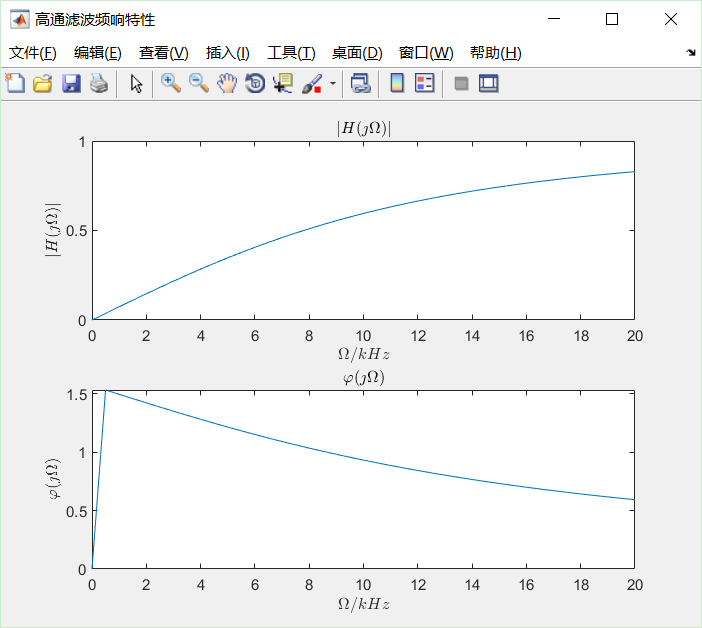
\includegraphics[width=\linewidth]{HP.png}
		\caption{高通滤波器频响特性曲线}
		\label{fig:高通滤波器频响特性曲线}
	\end{subfigure}
	\quad
	\begin{subfigure}[htpb]{.45\linewidth}
		\centering
		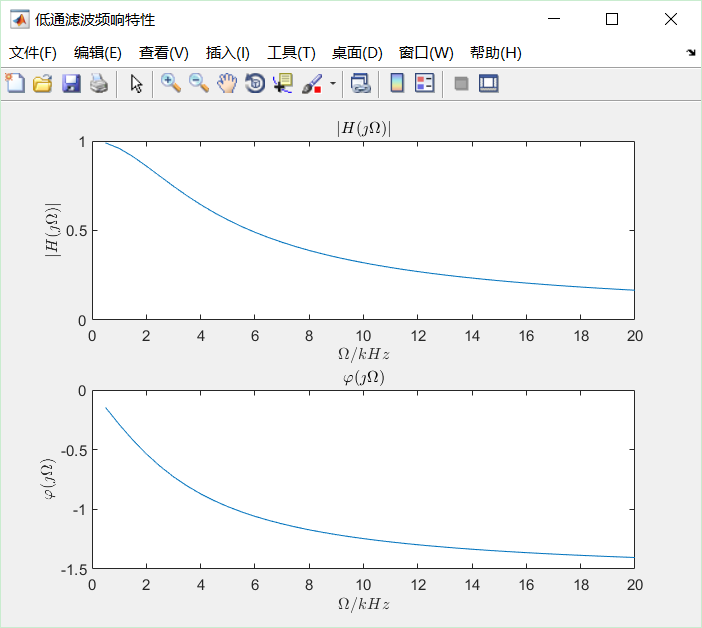
\includegraphics[width=\linewidth]{LP.png}
		\caption{低通滤波器频响特性曲线}
		\label{fig:低通滤波器频响特性曲线}
	\end{subfigure}
	\begin{subfigure}[htpb]{.45\linewidth}
		\centering
		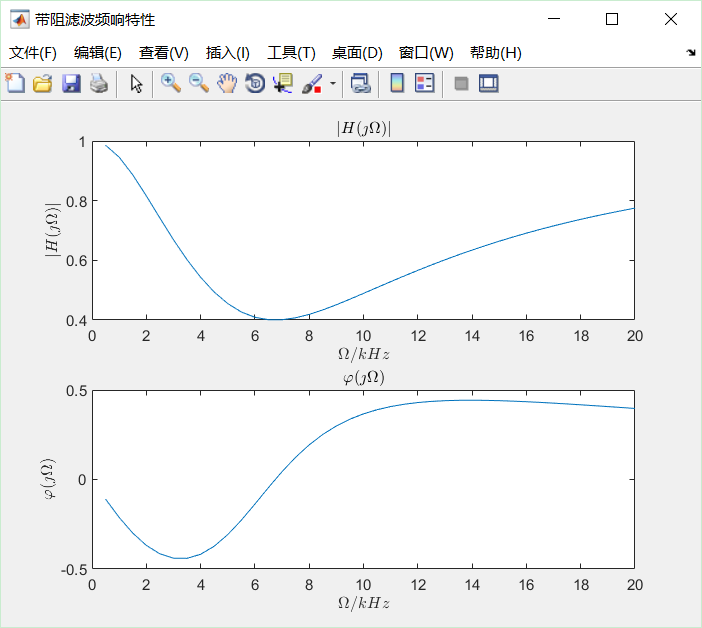
\includegraphics[width=\linewidth]{BS.png}
		\caption{带通滤波器频响特性曲线}
		\label{fig:带通滤波器频响特性曲线}
	\end{subfigure}
	\caption{频响特性曲线}
	\label{fig:频响特性曲线}
\end{figure}
\begin{Exercise}
	思考测量输入、输出信号相位差的具体方法。
\end{Exercise}
\begin{Answer}
	通过在双踪示波器器上测量。
\end{Answer}
\begin{Exercise}
	思考测试频率特性时,测试点频率应如何选取。
\end{Exercise}
\begin{Answer}
	测试点应在截止频率附近多选。
\end{Answer}
\section{实验原理图}%
\label{sec:实验原理图\arabic{chapter}}
\begin{figure}[htpb]
	\centering
	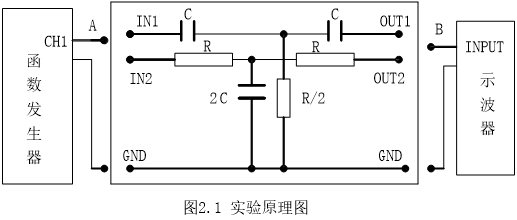
\includegraphics[width=0.8\linewidth]{2-4.png}
	\caption{实验原理图\arabic{chapter}}
	\label{fig:实验原理图\arabic{chapter}}
\end{figure}
图中:$ R=\SI{38}{k\ohm} $,$ C=\SI{3900}{pF} $,方框内为实验板上的电路。
\section{实验内容及步骤}%
\label{sec:实验内容及步骤\arabic{chapter}}
将信号源输出CH1的信号波形调为正弦波,信号的幅度调为$ V_\text{pp}=\SI{10}{V} $。
\subsection{RC高通滤波器的频响特性的测量}%
\label{sub:RC高通滤波器的频响特性的测量}
将信号源的输出端(A)接实验板的IN1端,滤波后的信号OUT1接示波器的输入(B) 。根据被测电路的参数及系统的频特性,将输入信号的频率从低到高逐次改变十 次以上(幅度保持$ V_\text{ipp}=\SI{10}{V} $) , 逐个测量输出信号的峰峰值大小($ V_\text{opp} $)及输出信号与输入信号的相位差 ,并将测量数据填入表\ref{tab:RC高通滤波器测量数据}:
\begin{figure}[htpb]
	\centering
	\begin{subfigure}[htpb]{.45\linewidth}
		\centering
		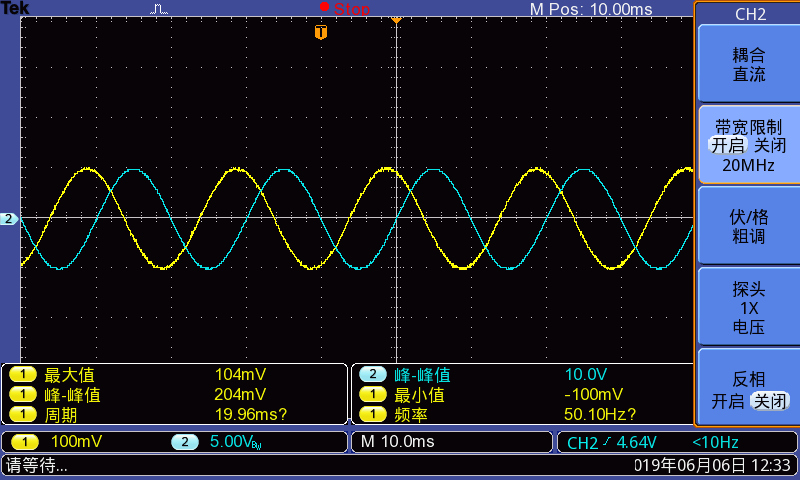
\includegraphics[width=\linewidth]{TEK21.png}
		\caption{RC高通滤波器测量数据\arabic{subfigure}}
		\label{fig:RC高通滤波器测量数据\arabic{subfigure}}
	\end{subfigure}
	\quad
	\begin{subfigure}[htpb]{.45\linewidth}
		\centering
		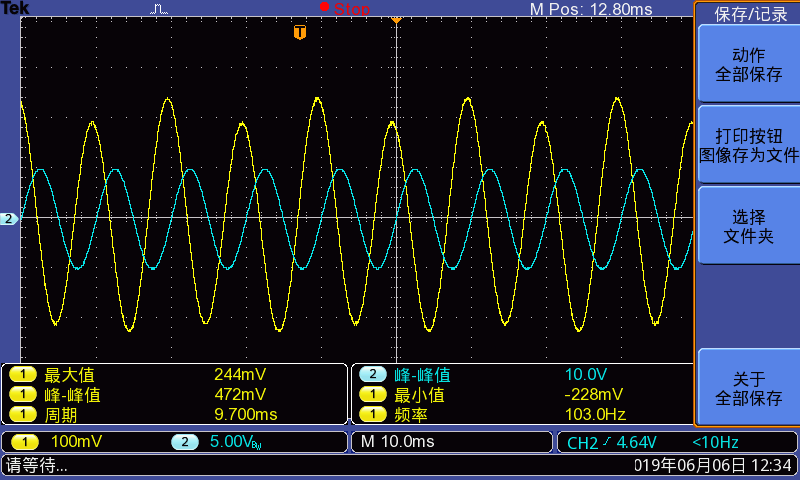
\includegraphics[width=\linewidth]{TEK22.png}
		\caption{RC高通滤波器测量数据\arabic{subfigure}}
		\label{fig:RC高通滤波器测量数据\arabic{subfigure}}
	\end{subfigure}
	\begin{subfigure}[htpb]{.45\linewidth}
		\centering
		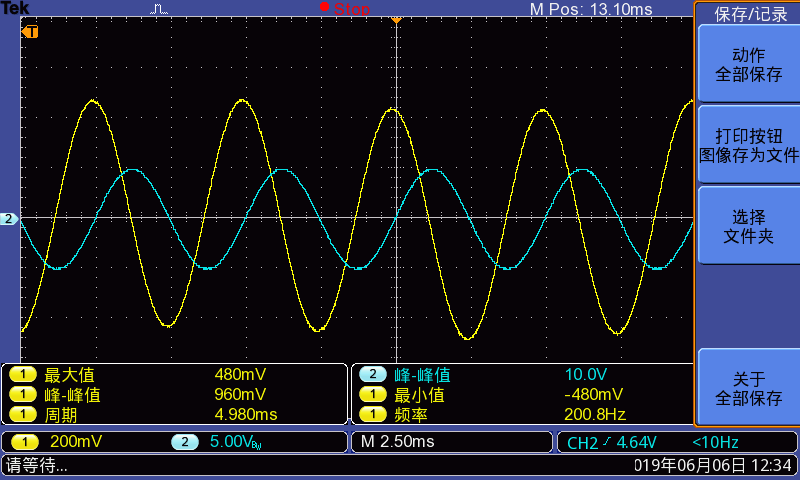
\includegraphics[width=\linewidth]{TEK23.png}
		\caption{RC高通滤波器测量数据\arabic{subfigure}}
		\label{fig:RC高通滤波器测量数据\arabic{subfigure}}
	\end{subfigure}
	\quad
	\begin{subfigure}[htpb]{.45\linewidth}
		\centering
		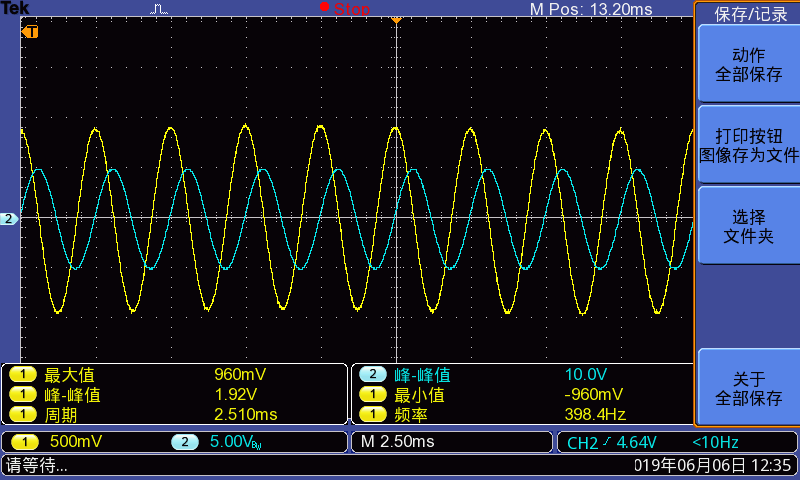
\includegraphics[width=\linewidth]{TEK24.png}
		\caption{RC高通滤波器测量数据\arabic{subfigure}}
		\label{fig:RC高通滤波器测量数据\arabic{subfigure}}
	\end{subfigure}
	\begin{subfigure}[htpb]{.45\linewidth}
		\centering
		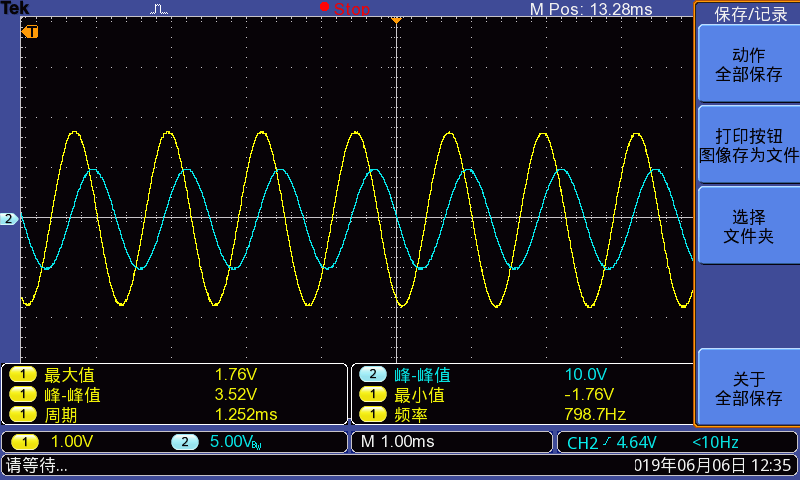
\includegraphics[width=\linewidth]{TEK25.png}
		\caption{RC高通滤波器测量数据\arabic{subfigure}}
		\label{fig:RC高通滤波器测量数据\arabic{subfigure}}
	\end{subfigure}
	\quad
	\begin{subfigure}[htpb]{.45\linewidth}
		\centering
		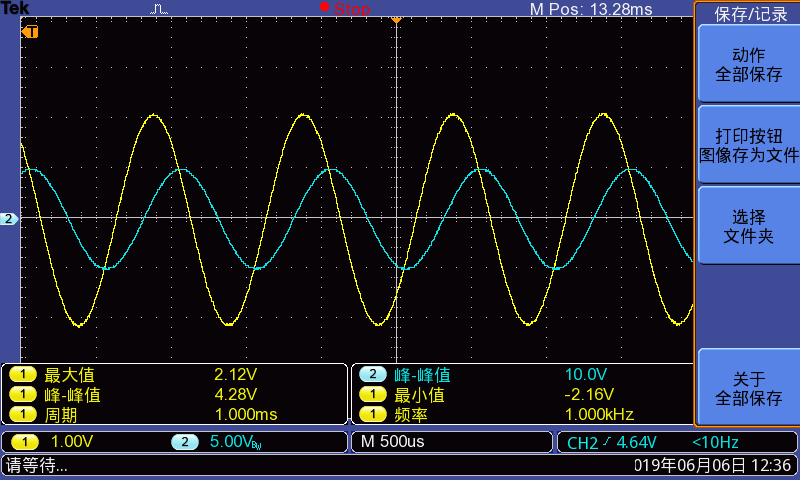
\includegraphics[width=\linewidth]{TEK26.png}
		\caption{RC高通滤波器测量数据\arabic{subfigure}}
		\label{fig:RC高通滤波器测量数据\arabic{subfigure}}
	\end{subfigure}
	\begin{subfigure}[htpb]{.45\linewidth}
		\centering
		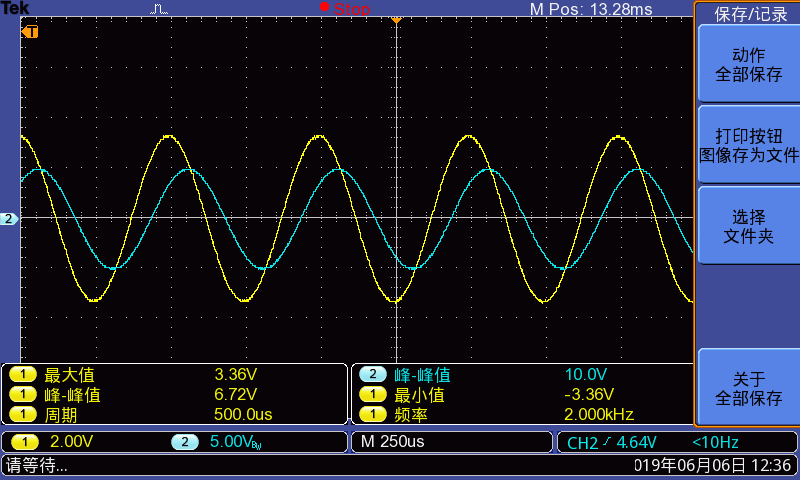
\includegraphics[width=\linewidth]{TEK27.png}
		\caption{RC高通滤波器测量数据\arabic{subfigure}}
		\label{fig:RC高通滤波器测量数据\arabic{subfigure}}
	\end{subfigure}
	\quad
	\begin{subfigure}[htpb]{.45\linewidth}
		\centering
		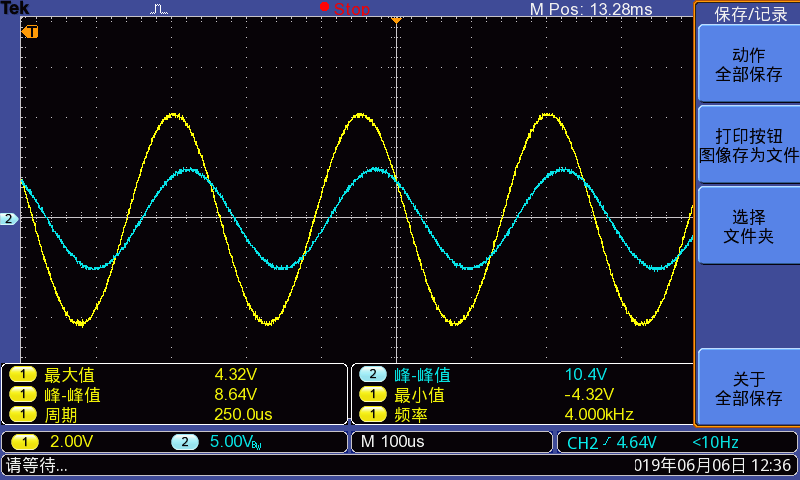
\includegraphics[width=\linewidth]{TEK28.png}
		\caption{RC高通滤波器测量数据\arabic{subfigure}}
		\label{fig:RC高通滤波器测量数据\arabic{subfigure}}
	\end{subfigure}
\end{figure}
\addtocounter{figure}{-1}
\begin{figure}[htpb]
	\setcounter{sub}{\value{subfigure}}
	\begin{subfigure}[htpb]{.45\linewidth}
		\setcounter{subfigure}{\value{sub}}
		\centering
		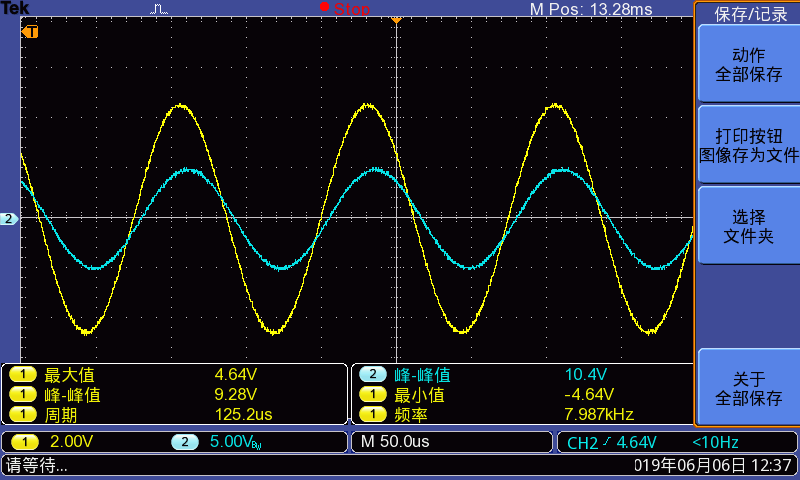
\includegraphics[width=\linewidth]{TEK29.png}
		\caption{RC高通滤波器测量数据\arabic{subfigure}}
		\label{fig:RC高通滤波器测量数据\arabic{subfigure}}
	\end{subfigure}
	\quad
	\begin{subfigure}[htpb]{.45\linewidth}
		\centering
		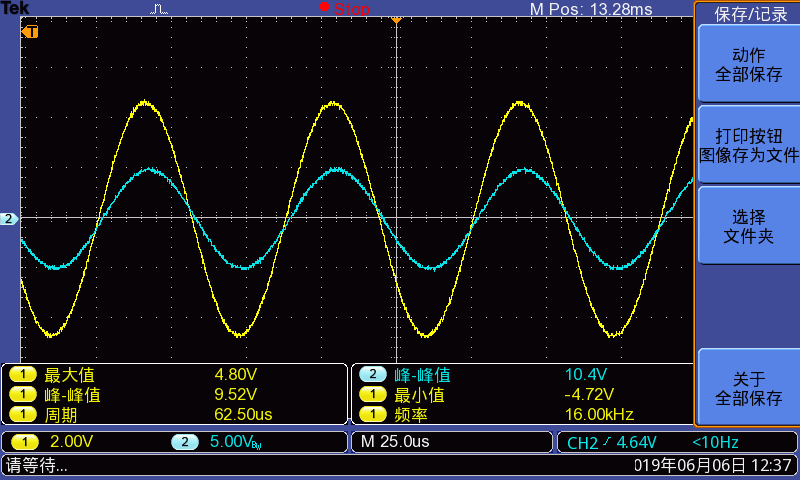
\includegraphics[width=\linewidth]{TEK2a.png}
		\caption{RC高通滤波器测量数据\arabic{subfigure}}
		\label{fig:RC高通滤波器测量数据\arabic{subfigure}}
	\end{subfigure}
	\caption{RC高通滤波器测量数据}
	\label{fig:RC高通滤波器测量数据}
\end{figure}
\begin{table}[htpb]
	\centering
	\caption{RC高通滤波器测量数据}
	\label{tab:RC高通滤波器测量数据}
	\csvreader[
	head to column names,
	tabular=|c|c|c|c|c|c|c|c|c|c|c|,
	table head=\hline,
	late after line=\\
	\hline
	]{src/2-5-1.csv}{}{ \a&\b&\c&\d&\e&\f&\g&\h&\i&\j&\k }
\end{table}
\subsection{RC低通滤波器的频响特性的测量}%
\label{sub:RC低通滤波器的频响特性的测量}
将信号源的输出(A)接实验板的IN2,滤波后的输出信号OUT2接示波器的输入(B)。根据被测电路的参数及系统的幅频特性,将输入信号的频率从低到高逐次改变十次以上(幅度保持$V_\text{ipp}=\SI{10}{V}$),逐个测量输出信号的峰峰值大小($V_\text{opp}$)及$\varphi(^{\circ})$,并将测量数据填入表\ref{tab:RC低通滤波器测量数据}:
\begin{table}[htpb]
	\centering
	\caption{RC低通滤波器测量数据}
	\label{tab:RC低通滤波器测量数据}
	\csvreader[
	head to column names,
	tabular=|c|c|c|c|c|c|c|c|c|c|c|,
	table head=\hline,
	late after line=\\
	\hline
	]{src/2-5-2.csv}{}{ \a&\b&\c&\d&\e&\f&\g&\h&\i&\j&\k }
\end{table}
\subsection{双TRC带阻滤波器的频响特性的测量}%
\label{sub:双TRC带阻滤波器的频响特性的测量}
将实验板上的两输入端IN1与IN2短接,输出端OUT1与OUT2短接;并将信号源的输出(A)接实验板输入(IN1)或(IN2),滤波后的输出OUT1或OUT2接示波器的输入(B)。根据被测电路的参数及系统的幅频特性,将输入信号的频率从低到高逐次改变二十次以上(幅度保持$ V_\text{ipp}=\SI{10}{V} $),逐个测量输出信号的峰峰值大小($ V_\text{opp} $)及$ \varphi(^{\circ}) $,并将测量数据填入表\ref{tab:双TRC带阻滤波器测量数据}:
\begin{table}[htpb]
	\centering
	\caption{双TRC带阻滤波器测量数据}
	\label{tab:双TRC带阻滤波器测量数据}
	\csvreader[
	head to column names,
	tabular=|c|c|c|c|c|c|c|c|c|c|c|,
	table head=\hline,
	late after line=\\
	\hline
	]{src/2-5-3.csv}{}{ \a&\b&\c&\d&\e&\f&\g&\h&\i&\j&\k }
\end{table}
\section{实验仪器及设备}%
\label{sec:实验仪器及设备\arabic{chapter}}
函数发生器一台 ,双踪示波器一台,实验板一块。
\section{实验报告要求}%
\label{sec:实验报告要求\arabic{chapter}}
\begin{Exercise}
	叙述实验内容及实验步骤。
\end{Exercise}
\begin{Answer}
	实验内容及实验步骤见第\ref{sec:实验内容及步骤\arabic{chapter}}节。
\end{Answer}
\begin{Exercise}
	整理实验数据,并以$ \lg f $为横坐标,$ V_{o}/V_{i} $为纵坐标,绘制三种滤波器的幅频特性曲线;以$ \lg f $为横坐标,$ \varphi(\Omega) $为纵坐标,绘制三种滤波器的相频特性曲线 。
\end{Exercise}
\begin{Answer}
	频响特性曲线见图\ref{fig:高通滤波实验波特图}。
\end{Answer}
\langCVfile[Matlab][code:lgfPlot.m][Matlab]{lgfPlot.m}{src/lgfPlot.m}
\langCVfile[Matlab][code:code272.m][Matlab]{code272.m}{src/code272.m}
\begin{figure}[htpb]
	\centering
	\matlablightfile{MATLAB Command Window}{src/code272.txt}
	\caption{运行界面}
	\label{fig:运行界面code272.m}
\end{figure}
\begin{figure}[htpb]
	\centering
	\begin{subfigure}[htpb]{.45\linewidth}
		\centering
		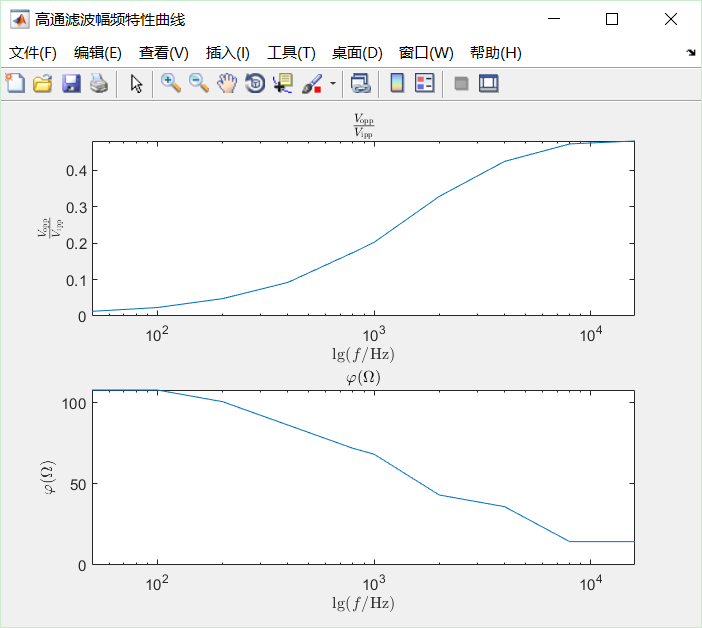
\includegraphics[width=\linewidth]{BodeHP.png}
		\caption{高通滤波实验波特图}
		\label{fig:高通滤波实验波特图}
	\end{subfigure}
	\quad
	\begin{subfigure}[htpb]{.45\linewidth}
		\centering
		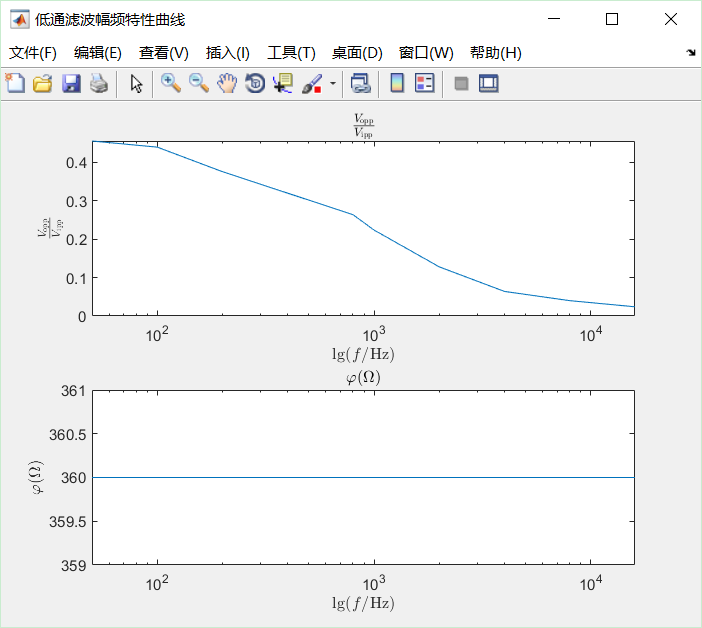
\includegraphics[width=\linewidth]{BodeLP.png}
		\caption{低通滤波实验波特图}
		\label{fig:低通滤波实验波特图}
	\end{subfigure}
	\begin{subfigure}[htpb]{.45\linewidth}
		\centering
		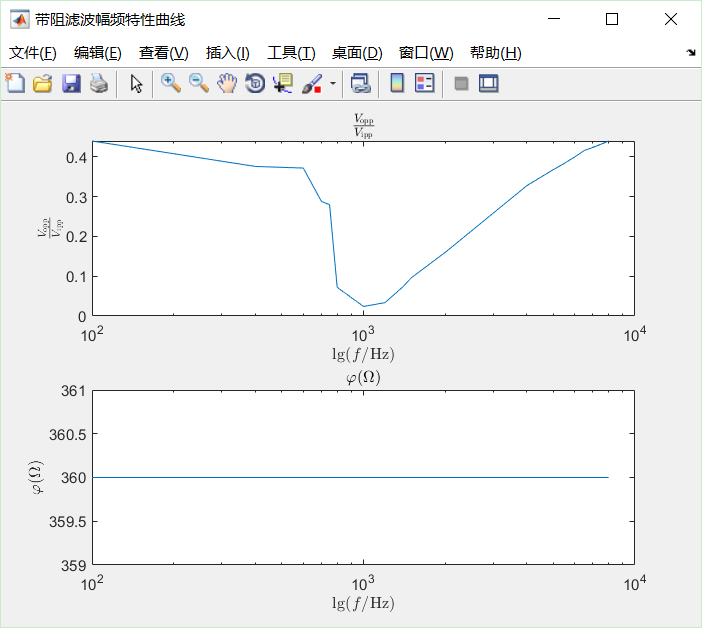
\includegraphics[width=\linewidth]{BodeBS.png}
		\caption{带阻滤波实验波特图}
		\label{fig:带阻滤波实验波特图}
	\end{subfigure}
	\caption{实验波特图}
	\label{fig:实验波特图}
\end{figure}
\begin{Exercise}
	将实验所得的频率响应特性曲线与仿真图进行比较;并将测得的各滤波器的截止频率与理论值进行比较,分析其结果是否一致,若误差较大则分析误差原因。
\end{Exercise}
\begin{Answer}
	仿真图见图\ref{fig:频响特性曲线}和\ref{fig:实验波特图},结果相对一致。
\end{Answer}

